\section{Considerações Iniciais}

Embora a refatoração dirigida a modelo tenha alcançado bastante reconhecimento e aceitação na literatura~\cite{Moghadam_2012,Maneerat_2011,Fourati_2011,Einarsson_2012,Steimann_2015,Akiyama_2011, Jensen_2010,Arendt_2012,Millan_2009,Tom_2008_2008}, ainda se faz necessário pesquisas nessa área~\cite{durelli_systematic_mapping, revisao_sistematica_uml_refactoring}.
Apesar da ADM, e principalmente o KDM tenham sido propostos para auxiliar todo o processo da modernização de sistemas, até esse momento existe uma carência de refatorações e ferramentas que auxiliem os modernizadores de software a aplicar refatorações de forma consistente para o metamodelo KDM. Neste contexto, no Capítulo~\ref{chapter:catalogo_refactoring_KDM} é descrito um conjunto de diretrizes pertinentes para auxiliar a criação de refatorações para o metamodelo KDM. Além disso, no Capítulo~\ref{chapter:catalogo_refactoring_KDM} também é apresentado uma adaptação do catálogo de refatoração do~\citeonline{Fowler1999} para o metamodelo KDM~\cite{durelli_catalogo}. O intuito da criação de refatorações para o metamodelo KDM é facilitar a condução da modernização de um determinado sistema legado utilizando a abordagem ADM.


Como já salientado nesta Tese, o OMG e a ADM fornecem um conjunto de metamodelos para auxiliar o engenheiro de modernização durante as atividades de modernização. Porém, hoje em dia a ADM não provê um metamodelo para auxiliar o engenheiro de modernização a promover o reúso de refatorações juntamente com os seus metamodelos padronizados durante o processo de modernização. 
Isso faz com que o engenheiro de modernização crie suas próprias soluções/refatorações. As refatorações criadas no Capítulo~\ref{chapter:catalogo_refactoring_KDM} não podem ser facilmente reutilizadas e compartilhadas entre os engenheiros de modernização. Com o intuito de suprir tal limitação no Capítulo~\ref{chapter:Toward_a_Refactoring_Metamodel_for_KDM} foi apresentado um metamodelo para auxiliar o engenheiro de modernização a promover o reúso de refatorações no contexto do metamodelo KDM. Com a utilização desse metamodelo, informações (metadados) sobre refatorações podem ser reutilizadas de forma independente de linguagem e plataforma. 

No Capítulo~\ref{chapter:Abordagem_de_sincronizacao} foi apresentado uma abordagem denominada KDM-SInc para manter instâncias do metamodelo KDM sincronizadas e consistentes após à aplicação de refatorações no KDM. Essa abordagem contém três principais passos: (\textit{i}) comparação (do ingles - \textit{diff}) entre a instância refatorada do metamodelo KDM e a instância do metamodelo KDM original, ou seja, a instância do metamodelo KDM antes do modernizador aplicar refatorações; (\textit{ii}) algoritmo de mineração para identificar todas as instâncias das metaclasses do KDM que possuem dependência com as metaclasses refatoradas e; (\textit{iii}) transformações pré-definidas em nível de modelo são aplicadas para propagar a mudança por todas as visões do KDM.

Como o objetivo de automatizar os conceitos apresentados nos Capítulos~\ref{chapter:catalogo_refactoring_KDM}, ~\ref{chapter:Toward_a_Refactoring_Metamodel_for_KDM} e~\ref{chapter:Abordagem_de_sincronizacao} neste capítulo é apresentado o apoio computacional denominado \sigla{KDM-RE}{\textit{Knowledge Discovery Model-Refactoring Environment}}. A ferramenta KDM-RE foi implementada como um conjunto de \textit{plug-ins} para o Ambiente de Desenvolvimento Eclipse IDE\footnote{\texttt{https://eclipse.org/home/index.php}}. Cada \textit{plug-in} representa um módulo da KDM-RE responsável por demonstrar a viabilidade dos conceitos descritos nos Capítulos~\ref{chapter:catalogo_refactoring_KDM}, ~\ref{chapter:Toward_a_Refactoring_Metamodel_for_KDM} e~\ref{chapter:Abordagem_de_sincronizacao}.  Nota-se que esse Capítulo é uma extensão do seguinte artigo: \textit{KDM-RE: A Model-Driven Refactoring Tool for KDM}~\cite{durelli_VEM_ferramenta}.

Os detalhes da KDM-RE estão apresentados nas seções que compõem este capítulo: a forma como a KDM-RE foi desenvolvida é descrita na Seção X\change{mudar}; na Seção Y é apresentado o módulo responsável por aplicar refatorações no metamodelo KDM; na Seção Z é apresentado o módulo responsável por instanciar o metamodelo SRM por meio de uma DSL, e também é apresentado como reutilizar programaticamente as refatorações persistidas no metamodelo SRM; na Seção X\change{mudar} é apresentado o módulo que implementa a abordagem KDM-SInc.



\section{Construção da KDM-RE}\label{sec:construcao_da_kdm_re}

A KDM-RE foi construída, de modo a ser utilizada em conjunto com os demais recursos oferecidos pelo ambiente de desenvolvimento Eclipse IDE. Os \textit{plug-ins} da KDM-RE são organizados em módulos de acordo com a sua funcionalidade. Os três principais módulos são:

\begin{itemize}
\item \textbf{Módulo de Refatoração}, que é responsável pela aplicação de refatorações de forma transparente em instâncias do metamodelo KDM;

\item \textbf{Módulo do SRM}, que é responsável pela instanciação e reúso do metamodelo SRM;

\item \textbf{Módulo de Sincronização}, que é responsável por manter consistente e programar mudanças após a aplicação de refatorações em instancias do metamodelo KDM.

\end{itemize}

A Figura~\ref{fig:arquitetura_ferramenta_kdm_re} apresenta uma visão lógica da arquitetura da ferramenta KDM-RE. Como observado a KDM-RE contém três camadas: (\textit{i}) IDE, (\textit{ii}) KDM-RE e (\textit{iii}) UI. A primeira camada da KDM-RE agrupa os recursos do Ambiente de Desenvolvimento Eclipse IDE para a criação dos três principais módulos da ferramenta KDM-RE. EMF, ATL, OCL, MoDisco, Papyrus, XText, EMFCompare e KDM são utilizadas durante a criação do KDM-RE.

\begin{figure}[h]
	\centering
	% Requires \usepackage{graphicx}
	\caption{Arquitetura da Ferramenta KDM-RE.}
	\label{fig:arquitetura_ferramenta_kdm_re}
	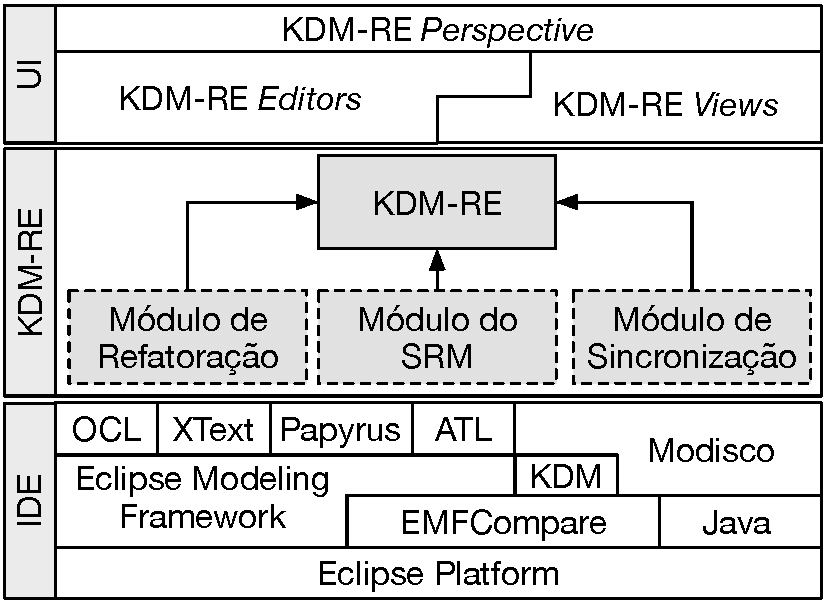
\includegraphics[scale=0.75]{images/arquitetura_KDM-RE}
	\fautor
\end{figure}

Na segunda camada é onde os módulos da KDM-RE são definidos. O módulo de refatoração utiliza EMF, ATL, OCL e MoDisco para criar um \textit{plug-in} onde o engenheiro de software pode aplicar refatorações em instâncias do metamodelo KDM. O módulo de sincronização implementa a abordagem KDM-SInc apresentada no Capítulo~\ref{chapter:Abordagem_de_sincronizacao}. Esse módulo utiliza o \textit{framework} EMFCompare e ATL. Por sua vez, o módulo do SRM utiliza EMF e XText. XText é utilizado no módulo do SRM para definir uma DSL para auxiliar a instanciação do metamodelo SRM. A última camada, UI, é responsável pela interface gráfica da ferramenta KDM-RE. Essa camada possui \textit{Wizards}, editores e visões para a aplicação, definição e reutilização das refatorações no contexto do KDM. Nas seções seguintes os três principais módulos da ferramenta KDM-RE são apresentados e discutidos.


\subsection{Módulo de Refatoração}

Nessa seção o módulo de refatoração é apresentado. Esse módulo foi implementado para prover suporte as refatorações criadas por meio das diretrizes apresentadas no Capítulo~\ref{chapter:catalogo_refactoring_KDM}. Na literatura é possível identificar um conjunto de técnicas e linguagens específicas para auxiliar a condução e especificação de transformação de modelos~\cite{Biehl_2010, Mens_2006, Allilaire_06}. Nesta Tese, a linguagem de transformação ATL~\cite{ATL_eclipse,Jouault_2008} foi escolhida para definir e aplicar refatorações no metamodelo KDM. Similarmente, as pre- e pós-condições foram implementadas em OCL. KDM-RE programaticamente executa as refatorações implementadas em ATL por meio da ATL EMF \textit{Transformation Virtual Machine}. As pre- e pós-condições são executadas na KDM-RE por meio da API Desden OCL\footnote{\texttt{http://www.dresden-ocl.org/}}. Essa API facilita a aplicação de OCL em qualquer metamodelo definido em EMF, no contexto desta Tese KDM. Como consequência, KDM-RE é capaz de suportar a detecção de violações semânticas estáticas em instâncias do metamodelo KDM.


Como já salientado no Capítulo~\ref{chapter:catalogo_refactoring_KDM} as refatorações foram definidas para serem executadas no contexto de instancias do metamodelo KDM. Dessa forma, é necessário primeiramente transformar um determinado sistema em instância do metamodelo KDM. Para tal, foi integrado a ferramenta MoDisco na KDM-RE como apresentado na Figura~\ref{fig:kdm_modisco_discovery}. Primeiramente, o engenheiro de software deve clicar com o botão direito em um projeto Java e escolher a opção \texttt{Knowledge Discovery} e em seguida escolher o menu \texttt{Discovery KDM MODEL}. MoDisco irá então transformar o código escrito na linguagem de programação Java para uma instancia do metamodelo KDM. 

\begin{figure}[h]
	\centering
	% Requires \usepackage{graphicx}
	\caption{KDM \textit{Discovery}.}
	\label{fig:kdm_modisco_discovery}
	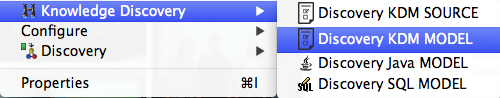
\includegraphics[scale=0.65]{images/kdm_discovery_kdm_re}
	\fautor
\end{figure}

Após a criação da instancia do metamodelo KDM o engenheiro de software pode aplicar as refatorações. A ferramenta KDM-RE permite que as refatorações sejam aplicadas por meio de duas interfaces gráficas. A primeira é uma extensão do editor gráfico da ferramenta MoDisco~\cite{Bruneliere_2014} que representa a instância do metamodelo em formato de árvore. A segunda interface gráfica é uma extensão do editor gráfico da ferramenta Papyrus\footnote{\texttt{https://eclipse.org/papyrus/}} que é uma ferramenta \sigla{CASE}{\textit{Computer-Aided Software Engineering}}. Por meio da segunda interface o engenheiro de software pode aplicar refatorações utilizando um diagrama de classe UML. Nota-se que nessa segunda interface de forma transparente as refatorações são de fato aplicadas em instâncias do KDM, o diagrama de classe UML é utilizado apenas como uma ponte entre as informações (nome de classe, atributos, métodos, etc) e as refatorações.

A primeira interface gráfica fornece uma visão de árvore da instância do metamodelo KDM (\textit{model browser}) como apresentado na Figura~\ref{fig:modisco_modeol_browser}. Lado esquerdo algumas das metaclasses (\texttt{ClassUnit}, \texttt{MethodUnit} e \texttt{StorableUnit}, etc) instanciadas do metamodelo KDM são apresentadas. Lado direito é onde as refatorações são aplicadas pelo engenheiro de software. Para aplicar as refatorações o engenheiro de software deve clicar com o botão direito em cima de uma determinada instância de metaclasse, por exemplo, \texttt{ClassUnit}, \texttt{MethodUnit}, \texttt{StorableUnit}, etc, assim, o menu \texttt{Refactoring KDM} irá aparecer como ilustrado na Figura~\ref{fig:kdm_re_refactoring_arvore}. Utilizando esse menu o engenheiro de software pode interagir com a instância do metamodelo KDM e escolher qual refatoração deve ser executada. Após o engenheiro de software clicar no menu \texttt{Refactoring KDM} e escolher uma determinada refatoração o processo se inicia. 

Para cada refatoração um determinado \textit{RefactoringWizard} é executado. Esse \textit{Wizard} irá guiar o engenheiro de software durante a aplicação da refatoração. Em cada refatoração a instância do metamodelo KDM deve ser analisada para identificar e obter os metadados das metaclasses que serão afetadas pela refatoração. Esses metadados são utilizadas tanto na ATL (refatoração) quanto na OCL (pré- e pós-condições). 


\begin{figure}[h]
	\centering
	% Requires \usepackage{graphicx}
	\caption{MoDisco \textit{Model Browser}.}
	\label{fig:modisco_modeol_browser}
	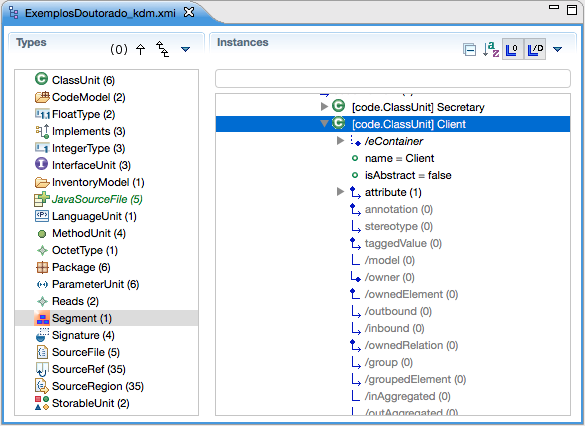
\includegraphics[scale=0.6]{images/kdm-re_modisco}
	\fautor
\end{figure}

\begin{figure}[h]
	\centering
	% Requires \usepackage{graphicx}
	\caption{KDM-RE \textit{Refactoring Browser}.}
	\label{fig:kdm_re_refactoring_arvore}
	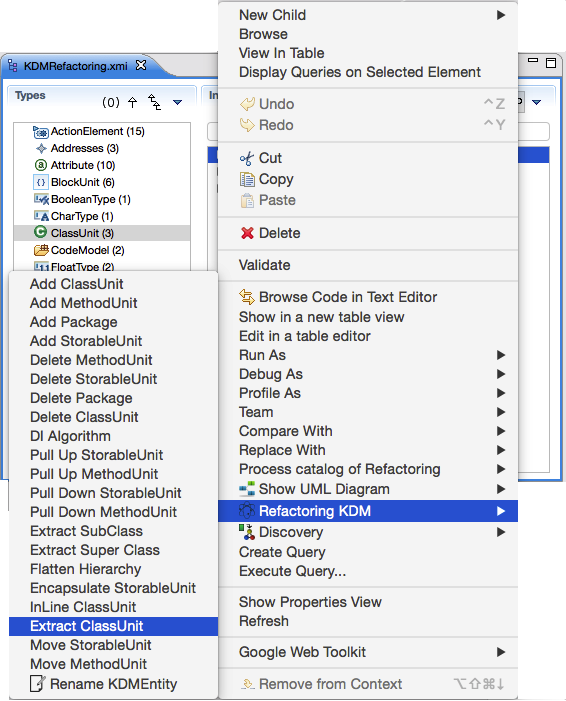
\includegraphics[scale=0.55]{images/novoMenuPopupKDM_RE}
	\fautor
\end{figure}


Por exemplo, suponha que o engenheiro de software identificou que uma instância da metaclasse \texttt{ClassUnit} está realizando o trabalho que deveria ser feita por duas instâncias (ver Figura~\ref{fig:kdm_re_wizard_extract_class}). Assim, o engenheiro de software deve aplicar a refatoração \texttt{Extract ClassUnit}. O primeiro passo é selecionar a instância da metaclasse \texttt{ClassUnit} para realizar a refatoração. Em seguida, deve-se selecionar a opção \texttt{Extract ClassUnit} no menu \texttt{Refactoring KDM}. Automaticamente KDM-RE irá criar um \textit{Wizard} para auxiliar o engenheiro de software como ilustrado na Figura~\ref{fig:kdm_re_wizard_extract_class}. Utilizando esse \textit{Wizard} o engenheiro de software define o nome da nova instância da metaclasse \texttt{ClassUnit}. Além disso, esse \textit{Wizard} permite visualizar todos as instâncias das metaclasses \texttt{StorableUnit} e \texttt{MethodUnit} que serão extraídas para a nova instância a ser criada. O \textit{Wizard} também permite especificar se instâncias da metaclasse \texttt{MethodUnit} devem ser criada para representar os métodos assessores (\textit{getters} e \textit{setters}). 

Uma característica importante da KDM-RE é a opção de visualizar previamente o resultado da refatoração. Assim, caso o engenheiro de software almejar visualizar o efeito da refatoração antes de efetivamente realiza-la o mesmo pode selecionar o botão \texttt{Preview}. Após clicar no botão \texttt{Preview} uma visão de comparação será criada como apresentado na Figura~\ref{fig:previa_resultado_extractClassUnit}. Essa visão de comparação contém duas principais partes. A parte superior representa quais instâncias foram deletadas, movidas e adicionadas de forma textual. Na parte inferior é possível visualizar graficamente a diferença entre as duas instâncias do metamodelo KDM, ou seja, a instância não refatorada (original) e a instância refatorada. O lado direito representa a instância do metamodelo KDM após a aplicação da refatoração \texttt{Extract ClassUnit} e o lado esquerdo representa a instância do metamodelo KDM antes da aplicação da refatoração. 

Como pode ser observado na Figura~\ref{fig:previa_resultado_extractClassUnit}, a instância direito do metamodelo KDM (instância refatorada) uma nova instância da metaclasse \texttt{ClassUnit} chamada \texttt{Document} foi criada - uma instância da metaclasse \texttt{StorableUnit} (\aspas{\texttt{CPF}}) foi movida para a nova \texttt{ClassUnit} \texttt{Document} - instâncias da metaclasse \texttt{MethodUnit} também foram criadas para representar os métodos assessores. A instância da metaclasse denominada \texttt{Pessoa} agora possui uma instância da metaclasse \texttt{StorableUnit} denominada \texttt{document} que representa um link entre as duas instâncias de \texttt{ClassUnit}.

\begin{figure}[h]
	\centering
	% Requires \usepackage{graphicx}
	\caption{\texttt{Extract ClassUnit} \textit{Wizard}.}
	\label{fig:kdm_re_wizard_extract_class}
	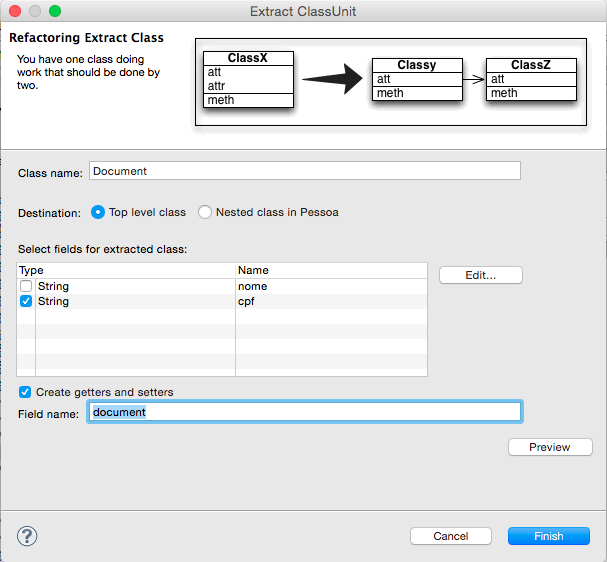
\includegraphics[scale=0.5]{images/extractClassEasierToExplainerEMFCOmpare}
	\fautor
\end{figure}

\begin{figure}[h]
	\centering
	% Requires \usepackage{graphicx}
	\caption{Prévia do resultado da refatoração \texttt{Extract ClassUnit}.}
	\label{fig:previa_resultado_extractClassUnit}
	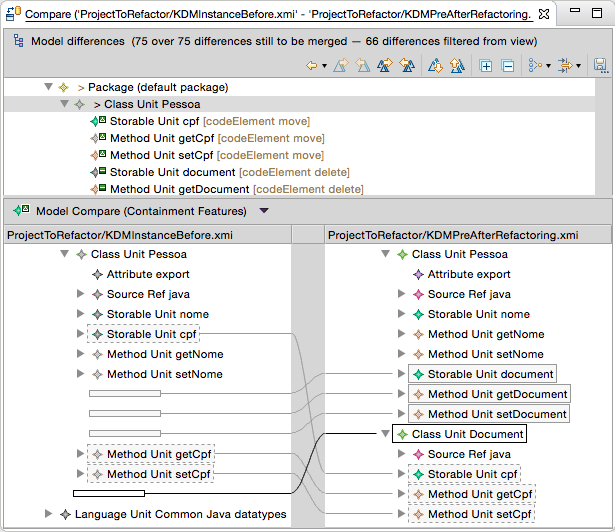
\includegraphics[scale=0.5]{images/previaRefatoracaoExtractClassUnitEMFCOmpare}
	\fautor
\end{figure}


Após especificar todas as entradas necessárias e visualizar o efeito que a refatoração irá resultar na instância do metamodelo KDM o engenheiro de software deve clicar no botão \textit{Finish}. A KDM-RE executa a API Dresden OCL para verificar as pré-condições. Caso as pré-condições forem satisfeitas a refatoração \texttt{Extract ClassUnit} é executada efetivamente. A execução da refatoração é totalmente realizada com base na ATL. As entradas informadas pelo engenheiro de software no \textit{Wizard} são enviadas para ATLs pré-definidas e em seguida são executadas programaticamente pela KDM-RE por meio da ATL EMF \textit{Transformation Virtual Machine}\footnote{\texttt{https://wiki.eclipse.org/ATL/EMFTVM}}. Em seguida, a KDM-RE  executa a API Dresden OCL para verificar as pós-condições. 


Embora a primeira interface gráfica seja útil para aplicar refatorações diretamente em instâncias do metamodelo KDM, a mesma não é intuitiva. Dessa forma, a segunda interface gráfica tem como objetivo deixar as refatorações mais fáceis e intuitivas de serem aplicadas. Por exemplo, embora~\citeonline{Fowler1999} tenha criado um catálogo de refatorações para ser utilizado em código-fonte, mais de 60\% das refatorações (44 de 72) são ilustradas utilizando modelos, mais especificadamente diagramas de classes da UML. Além disso, ~\citeonline{Zhang_2005, Boger_2003} afirmam que algumas refatorações, por exemplo, \texttt{Extract Method}, são mais naturais quando executadas diretamente no código-fonte. Enquanto que outras refatorações, como: \texttt{Rename Class}, \texttt{Pull Up Method}, \texttt{Push Down Method}, etc, podem ser aplicadas tanto em código-fonte quando em modelos; já as refatorações que lidam com herança, tais como \texttt{Extract Class}, \texttt{Extract Interface}, \texttt{Replace Inheritance with Delegation}, são mais intuitivas quando aplicadas diretamente em nível de modelo, tais como diagrama de classe da UML. 

Neste contexto, a KDM-RE foi integrada com a ferramenta CASE Papyrus para utilizar o diagrama de classe da UML. Para utilizar essa segunda interface primeiramente é necessário transformar a instância do metamodelo KDM para uma instância da UML. Assim, as refatorações definidas na KDM-RE podem ser aplicadas diretamente em diagramas da UML, por exemplo, pode-se aplicar refatorações por meio do diagrama de classe. É importante observar que embora as refatorações sejam aplicadas graficamente por meio do diagrama de classe da UML todas as refatorações (transformações) são aplicadas transparentemente na instância do metamodelo KDM e não na instância da UML - apenas informações são extraídas do diagrama de classe da UML e são enviados como entrada para as refatorações pré-definida em ATL. %Tecnicamente essa segunda interface é implementada como uma extensão da ferramenta CASE Papyrus.


Os passos para utilizar a segunda interface são similares a primeira interface. Porém, um passo a mais se faz necessário para utilizar a segunda interface. Deve-se gerar uma instância do metamodelo UML tendo como base uma instância do metamodelo KDM. A geração da instância do metamodelo UML é totalmente apoia por um \textit{plug-in} denominado \texttt{DiscoverUmlModelFromKdmModel} do MoDisco. Esse \textit{plug-in} utiliza regras ATL para criar uma instância do metamodelo UML tendo como base outra instância do metamodelo KDM. Por exemplo, na Figura~\ref{fig:kdmToUML} são apresentadas duas instâncias dos metamodelos UML (lado esquerdo) e KDM (lado direito) após a transformação, respectivamente.

\begin{figure}[!h]
	\centering
	% Requires \usepackage{graphicx}
	\caption{Instância UML gerada a partir do KDM.}
	\label{fig:kdmToUML}
	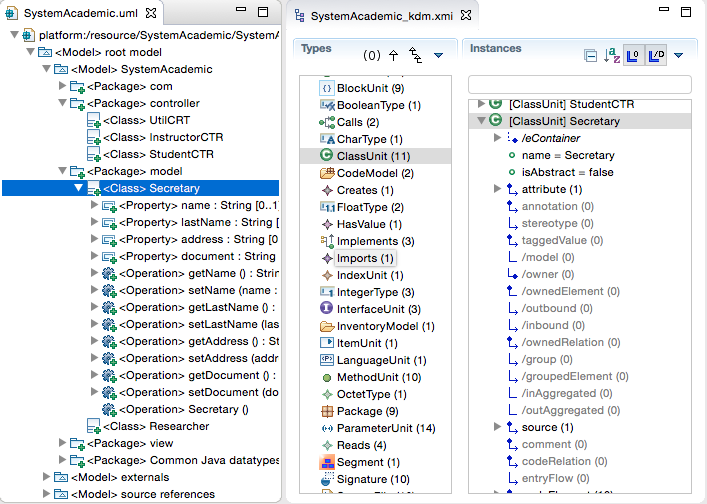
\includegraphics[scale=0.5]{images/kdmToUML}
	\fautor
\end{figure}

Após a criação da instância do metamodelo UML o próximo passo é utilizar a ferramenta CASE Papyrus para exibir a nova instância do metamodelo UML por meio do diagrama de classe como apresentado na Figura~\ref{fig:kdmToUML_diagrama_de_classe}. Por meio desse diagrama a KDM-RE permite que o engenheiro de software realize refatorações. Por exemplo, na Figura~\ref{fig:refatoracao_papyrus_KDM_iteragir} é ilustrado que primeiramente o engenheiro de software deve clicar com o botão direito em cima do elemento que almeja refatorar, nesse caso a classe \texttt{Secretary}, escolher a opção \texttt{Refactoring Model} e em seguida decidir qual refatoração aplicar, nesse exemplo - \texttt{Extract ClassUnit}. Em seguida um \textit{RefactoringWizard} similar ao apresentado na Figura~\ref{fig:kdm_re_wizard_extract_class} é executado. O mesmo também irá guiar o engenheiro de software durante a aplicação da refatoração. Da mesma forma como na primeira interface, na segunda interface o engenheiro de software pode solicitar também a realização de uma prévia da refatoração. O resultado dessa solicitação será uma interface similar a apresentada na Figura~\ref{fig:previa_resultado_extractClassUnit}.

\begin{figure}[!h]
	\centering
	% Requires \usepackage{graphicx}
	\caption{Diagrama de Classe da UML gerada a partir do KDM.}
	\label{fig:kdmToUML_diagrama_de_classe}
	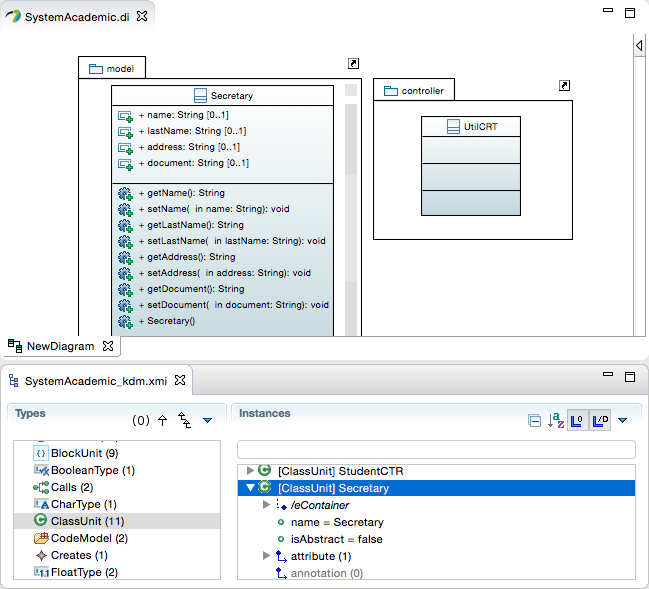
\includegraphics[scale=0.5]{images/refatoracao_UML_papyrus}
	\fautor
\end{figure}

As informações fornecidas pelo engenheiro de software no \textit{Wizard} são enviadas para ATLs pré-definidas e em seguida são executadas programaticamente pela KDM-RE por meio da ATL EMF \textit{Transformation Virtual Machine}. O resultado da refatoração altera a instância do metamodelo KDM e é replicado automaticamente no diagrama de classe da UML, portanto, o engenheiro de software pode visualizar graficamente no diagrama de classe UML o resultado da refatoração.

\begin{figure}[!h]
	\centering
	% Requires \usepackage{graphicx}
	\caption{Refatorações por meio do Diagrama de Classe.}
	\label{fig:refatoracao_papyrus_KDM_iteragir}
	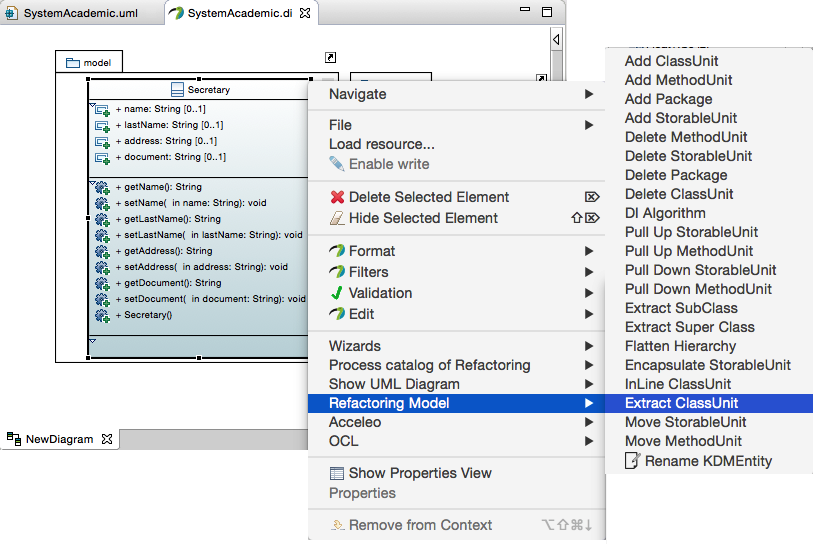
\includegraphics[scale=0.5]{images/kdm_uml_papyrus_refactoring_extract_class_new}
	\fautor
\end{figure}

\section{Módulo do SRM}\label{label:sec_modulo_do_srm}

Nessa seção é apresentado um módulo desenvolvido para fornecer suporte ao metamodelo SRM apresentado no Capítulo~\ref{chapter:Toward_a_Refactoring_Metamodel_for_KDM}  Figura~\ref{fig:meta_modelo_SRM}. Esse módulo implementa o metamodelo SRM utilizando EMF por meio do meta-metamodelo Ecore. Nesse módulo também foi definido uma linguagens específica de domínio (DSL) para facilitar a instanciação do metamodelo SRM. A gramática dessa DSL é apresentada no Capítulo~\ref{chapter:Toward_a_Refactoring_Metamodel_for_KDM}, mais detalhadamente nos Códigos-fontes~\ref{lst:dsl_part_1}, \ref{lst:dsl_part_2}, \ref{lst:dsl_part_3}, \ref{lst:dsl_part_4} e \ref{lst:dsl_part_5}.


Esse módulo fornece uma forma de compartilhar e reutilizar refatorações por meio de instâncias do metamodelo SRM. Para permitir o reúso e compartilhamento de refatorações um repositório remoto foi criado. Esse repositório remoto é dedicado para executar solicitações RESTful. Instâncias do metamodelo SRM são enviadas e recebidas por meio da API RESTful. Isso é possível pois as instâncias do SRM são arquivos que persistidos no formato XMI. \sigla{JPA}{Java Persistence API} e o banco de dados MySQL foram utilizados para realizar as persistências das instâncias do metamodelo SRM.

%Para utilizar as vantagens dos metamodelo SRM, os engenheiros de modernização precisam ter conhecimento de linguagem de programação avançada. Eles devem estar familiarizados como as semânticas das refatorações (por exemplo, qual(is) é (são) o(s) pré-requisito(s) para a execução de uma refatoração) e como/onde utilizar e programar tais refatorações. Além disso, a instanciação de uma refatoração utilizando o metamodelo SRM é bastante verbosa, complexa e propensa a erros, pois exige conhecimento avançadas de refatoração e habilidades de programação em relação a API Ecore/EMF. Como salientado no Capítulo~\ref{chapter:Toward_a_Refactoring_Metamodel_for_KDM} o metamodelo SRM foi desenvolvido para permitir a reutilização de metaclasses já definidas no metamodelo KDM. Mais especificadamente os elementos estruturais que são utilizados em uma refatoração são representados por metaclasses previamente já definidas no metamodelo KDM, tais como: \texttt{ClassUnit}, \texttt{InterfaceUnit}, \texttt{Package}, \texttt{StorableUnit}, etc.

%No Código-fonte~\ref{cod:instancia_do_SRM} é apresentado um trecho onde é feita a instanciação em memória de algumas metaclasses definidas no metamodelo SRM. Note que nesse código-fonte a instanciação das metaclasses do metamodelo SRM é um processo verboso e propenso a erros. Para instanciar o metamodelo SRM o engenheiro deve saber utilizar a API do \textit{framework} EMF. Metaclasses são instanciadas em EMF utilizando o conceito de fabrica (em inglês - \textit{Factory}). Cada fabrica de uma metaclasse possui um método \texttt{createX}, onde X representa o nome da metaclasse do metamodelo. Para criar uma instancia válida do metamodelo SRM o engenheiro de modernização deve seguir um conjunto de passos. Por exemplo, como pode ser observado na linha 1 do Código-fonte~\ref{cod:instancia_do_SRM} uma instância da metaclasse \texttt{Author} é criada por meio da interface \texttt{RefactoringModelFactory} e do método \texttt{createAuthor()}. Em seguida, todos os meta-atributos da metaclasse \texttt{Author} devem ser especificados como apresentado nas linhas 2 e 3 do Código-fonte~\ref{cod:instancia_do_SRM}. Nas linhas 4-14 outras metaclasses do metamodelo SRM são instanciadas. 


%Como apresentado e salientado no Capítulo~\ref{chapter:Toward_a_Refactoring_Metamodel_for_KDM} a instanciação de uma refatoração por meio do SRM pode ser um processo demorado e suscetível a erro. Para diminuir a quantidade de código-fonte, esforço obrigatórios e competência necessárias para instanciar refatorações utilizando o metamodelo SRM, a KDM-RE provê uma DSL que auxilia a instanciação de refatorações sistematicamente. Na parte superior a esquerda da Figura~\ref{fig:DSL_SRM} é possível visualizar o relacionamento entre a DSL criada e as metaclasses do metamodelo SRM. 

Por meio das gramáticas apresentadas nos Códigos-fontes~\ref{lst:dsl_part_1}, \ref{lst:dsl_part_2}, \ref{lst:dsl_part_3}, \ref{lst:dsl_part_4} e \ref{lst:dsl_part_5} Xtext gera um editor textual para o ambiente de desenvolvimento Eclipse IDE. Esse editor textual provê \textit{highlighting} de sintaxe, \textit{autocomplete} de código e navegação de código. Na parte superior a esquerda da Figura~\ref{fig:DSL_SRM} é possível visualizar trechos da DSL resultante. Além disso, essa figura ilustra o relacionamento entre a DSL criada e as metaclasses do metamodelo SRM, ou seja, representa que a sintaxe da DSL esta em conformidade com as metaclasses do SRM.

%\begin{codigo}[caption={[Instanciação do metamodelo SRM programaticamente.] Instanciação do metamodelo SRM.},escapeinside={(*@}{@*)}, basicstyle=\footnotesize, label={cod:instancia_do_SRM}, language=Java]{Name}
%Author author = RefactoringModelFactory.eINSTANCE.createAuthor();
%author.setName("Rafael");
%author.setLastName("Durelli");
%RefactoringModel rM = RefactoringModelFactory.eINSTANCE.createRefactoringModel();
%rM.setAuthor(author);
%RefactoringLibrary library = RefactoringModelFactory.eINSTANCE.createRefactoringLibrary();
%lib.setName("Fowler's refactorings");
%lib.setDescription("Contains some Fowler's refactorings such as ExtractClass, RenameElements, PushMethod, PushAttribute, etc.");
%lib.setShortDescription("Fine grained Refactorings");
%rM.getLibraries().add(lib);
%Catalog cat = RefactoringModelFactory.eINSTANCE.createCatalog();
%cat.setAuthor(author);
%cat.setName("Fowler's catalog");
%libr.getCatalogs().add(cat);
%...
%\end{codigo}

\begin{figure}[!h]
	\centering
	% Requires \usepackage{graphicx}
	\caption{DSL para auxiliar a instanciação do SRM.}
	\label{fig:DSL_SRM}
	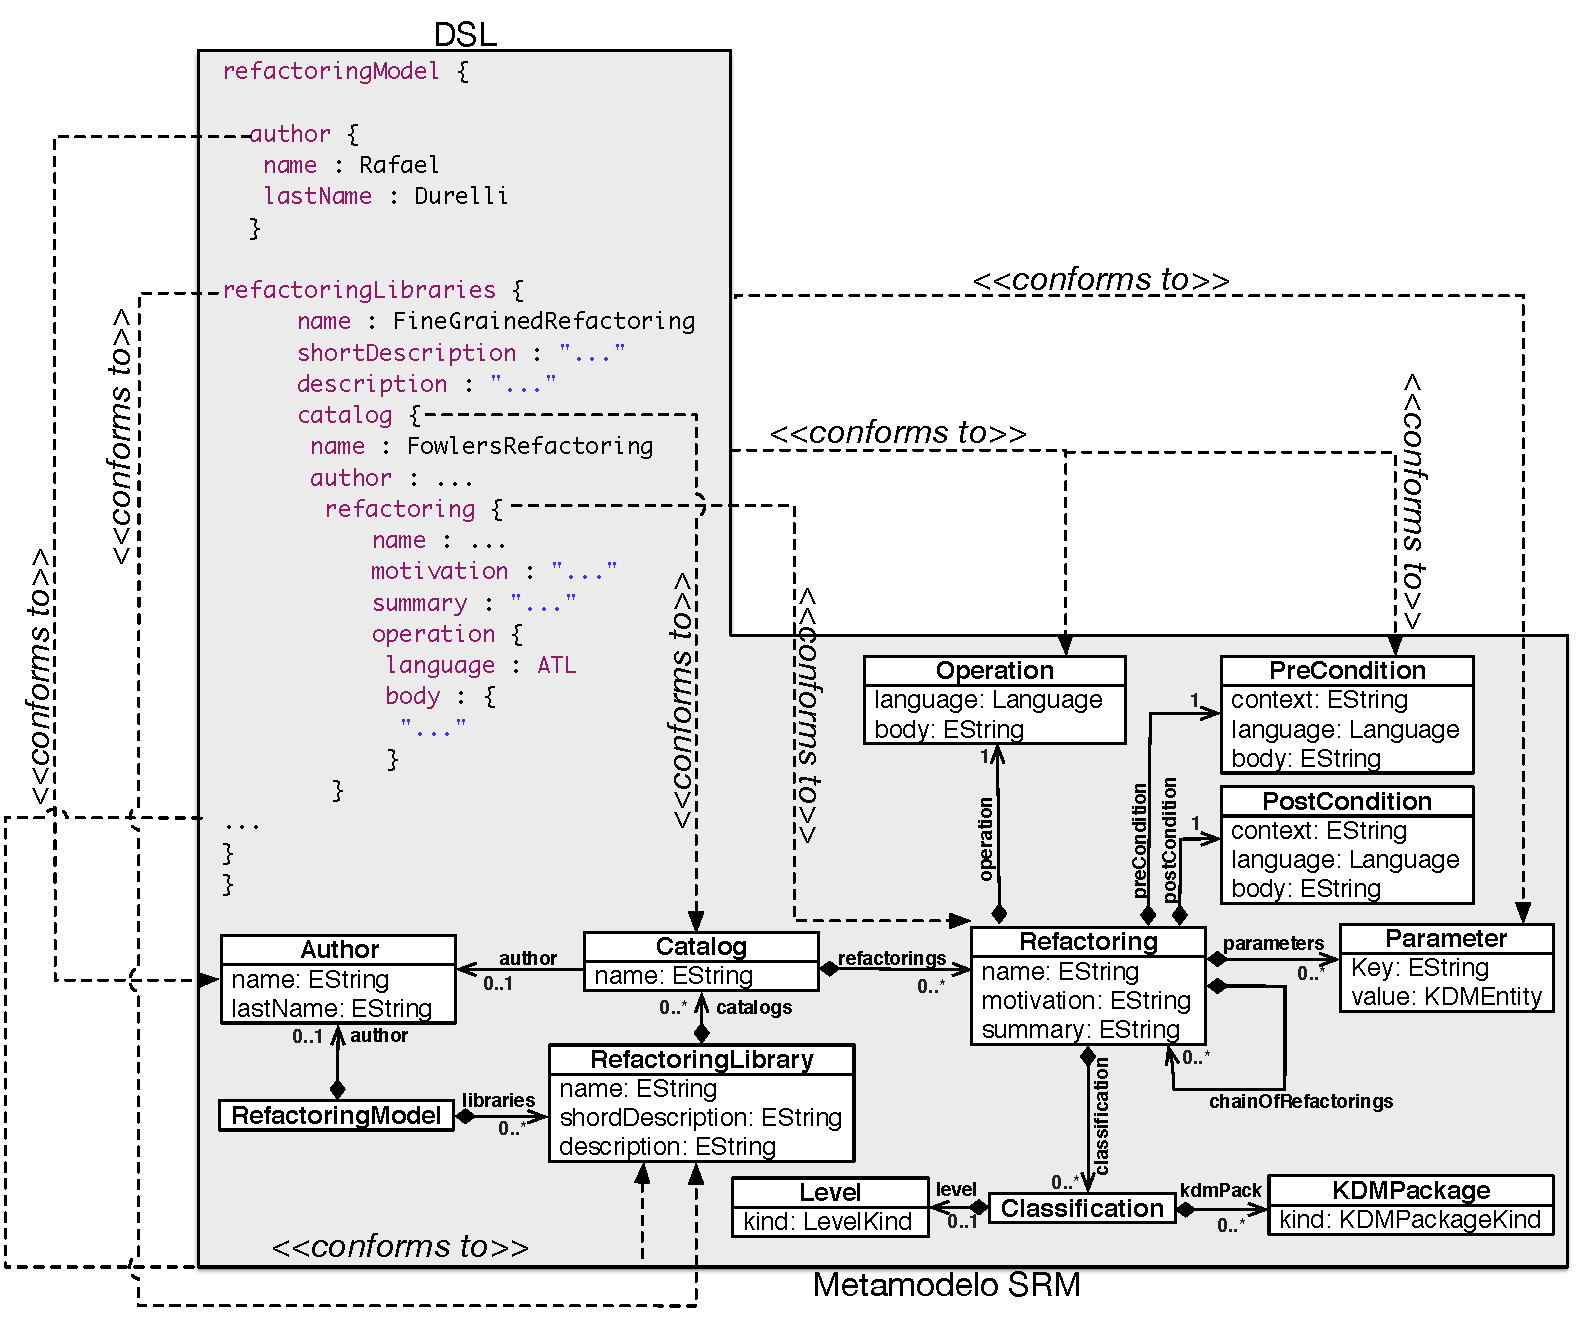
\includegraphics[scale=0.6]{images/MetaModelEDSL}
	\fautor
\end{figure}

Cada trecho de código da DSL representa uma instancia de uma metaclasse do metamodelo SRM, ou seja, cada declaração da DSL está em conformidade com uma metaclasse do SRM. Por exemplo, a palavra-chave \texttt{refactoringModel} \texttt{author} entre \aspas{\{} e \aspas{\}} representa a instanciação da metaclasse \texttt{Author} do SRM que possui dois meta-atributos: \texttt{name} e \texttt{lastName}. A DSL criada para auxiliar a instanciação do SRM foi desenvolvida utilizando Xtext\footnote{\texttt{https://www.eclipse.org/Xtext/}}. Xtext é um \textit{framework} do Eclipse\footnote{\texttt{https://www.eclipse.org}} que facilita a definição de gramática\footnote{Gramáticas representam a definição formal de um sintaxe textual concreta. Consistem em um conjunto de regras de produção para definir como o \textit{textual input} (ou seja, sentenças) são representadas. Basicamente, as regras de produção podem ser representadas utilizando \sigla{BNF}{\textit{Backus–Naur Form}}, por exemplo, \textit{S ::= P1 ... Pn}, essa gramática define um símbolo \textit{S} por um conjunto de expressões \textit{P1 ... Pn}.} 
com a utilização de um metamodelo que foi definido utilizando EMF. Xtext tem como principal objetivo automatizar e agilizar o processo de desenvolvimento de DSLs. Note que a sintaxe da DSL segue as terminologias e conceitos definidos no metamodelo SRM para facilitar a utilização da DSL e o entendimento do metamodelo SRM.

%Em Xtext a gramática segue uma notação similar ao \textit{Backus–Naur Form} (BNF) chamada de regras do \textit{parser}. Tais regras representam a sintaxe concreta da DSL. Note que para facilitar o entendimento da DSL, trechos da mesma são mostradas em listagens de códigos separados, bem como símbolos para explanar o propósito de uma terminada linha da gramática. No Código-fonte~\ref{lst:dsl_part_1} é ilustrado o primeiro trecho da gramática concreta da DSL desenvolvida. A gramática começa com a definição do nome da DSL (SRM) (ver Código-fonte~\ref{lst:dsl_part_1} \ding{182}). Em sequência é definido os metamodelos que devem ser importados para serem utilizados durante a criação da DSL: o metamodelo SRM\ding{183} e o Ecore\ding{184}.


%\begin{lstlisting}[language=Xtext, frame=single, basicstyle={\scriptsize}, mathescape=true, label={lst:dsl_part_1}, caption={Gramática da DSL - parte 1}]
%$\textrm{\ding{182}}$ grammar refactoring.xtext.SRM with org.eclipse.xtext.common.Terminals 
%$\textrm{\ding{183}}$ import platform:/resource/refactoring/model/SRM.ecore
%$\textrm{\ding{184}}$ import http://www.eclipse.org/emf/2002/Ecore as ecore
%RefactoringModel: 
%	$\textrm{\ding{185}}$ `refactoringModel' name = ID `{'
%	$\textrm{\ding{186}}$ author = Author
%	$\textrm{\ding{187}}$ libraries += RefactoringLibrary$^{*}$;
%	`}'
%\end{lstlisting}


%Em seguida é criado a primeira regra. Essa regra começa com a definição da metaclasse \texttt{RefactoringModel}. O corpo da regra começa logo após os \aspas{\texttt{:}}. Primeiramente para o entendimento da regra, é importante destacar que literais de \textit{string} (em Xtext os literais podem ser expressos com aspas simples ou duplas) definem palavras-chave da DSL. Como pode ser observado no Código-fonte~\ref{lst:dsl_part_1} é esperado a palavra-chave \texttt{refactoringModel}\ding{185} seguido por um \texttt{ID} e \aspas{\{}. A gramática que rege o objeto \texttt{ID} é definida como uma sequência ilimitada de maiúsculas e minúsculas, números e o carácter de sublinhado, embora possa não começa por um dígito. A gramática que representa o nó \texttt{ID}\ding{182} pode ser visualizada no Código-fonte~\ref{lst:dsl_part_2}. 

%\begin{lstlisting}[language=Xtext, frame=single, basicstyle=\scriptsize, mathescape=true, label={lst:dsl_part_2}, caption={Gramática da DSL - parte 2}]
%	$\textrm{\ding{182}}$ terminal ID: (`a'..`z' | `A'..`Z'|`_')(`a'..`z' | `A'..`Z'|`_'|`0'..`9')*;
%\end{lstlisting}

%Ainda no Código-fonte~\ref{lst:dsl_part_1} a expressão \texttt{author=Author}\ding{186} especifica que pode-se instanciar uma instancia da metaclasse \texttt{Author}. A expressão \texttt{(libraries += RefactoringLibrary)$^{*}$}\ding{187} descrita no Código-fonte~\ref{lst:dsl_part_1} especifica que pode-se instanciar várias instâncias da metaclasse \texttt{RefactoringLibrary}. O operador estrela, \aspas{\texttt{*}}, ilustra que o número de elementos (nesse caso \texttt{RefactoringLibrary}) é arbitrário; em particular, ele pode ser qualquer número \texttt{>=} 0. Operador \texttt{+=} por sua vez representa que a propriedade \texttt{libraries} será uma lista do tipo \texttt{RefactoringLibrary}.

%\begin{lstlisting}[language=Xtext, frame=single, basicstyle=\scriptsize, mathescape=true, label={lst:dsl_part_3}, caption={Gramática da DSL - parte 3}]
%Author:
%	$\textrm{\ding{182}}$ `author' `{'
%	$\textrm{\ding{183}}$ `name' `:' name = ID  
%		$\textrm{\ding{229} \ding{184}}$ `lastName' `:' lastName = ID; 
%`}'
%RefactoringLibrary:
%	$\textrm{\ding{185}}$ `refactoringLibraries' `{'
%	$\textrm{\ding{186}}$ `name' `:' name = ID  
%		$\textrm{\ding{229}}$ `shortDescription' `:' shortDescription = STRING
%		$\textrm{\ding{229}}$ `description' `:' description = STRING
%		$\textrm{\ding{229}}$ $\textrm{\ding{187}}$ catalogs += Catalog$^{*}$
%`}'
%\end{lstlisting}

%A definição das regras que regem as metaclasses \texttt{Author} e \texttt{RefactoringLibrary} são apresentadas no Código-fonte~\ref{lst:dsl_part_3}. A regra para a definição de \texttt{Author} começa com a definição da palavra-chave \texttt{author} seguida por um \aspas{\{}\ding{182}. Em seguida a palavra-chave \texttt{name} é esperada, seguido por \aspas{\texttt{:}} \ding{183}. Posteriormente a palavra-chave \texttt{lastName} também é esperada, seguido por \aspas{\texttt{:}} \ding{184}. Na linha 6 do Código-fonte~\ref{lst:dsl_part_3} começa a definição da regra da metaclasse \texttt{RefactoringLibrary}. A regra para a definição de \texttt{RefactoringLibrary} começa com a definição da palavra-chave \texttt{refactoringLibraries} seguida por um \aspas{\{}\ding{185}. Em seguida, deve-se especificar a palavra-chave \texttt{name} e \texttt{:}. Posteriormente, as palavras-chaves \texttt{shortDescription} e \texttt{description} são especificadas nas linhas 9 e 10, respectivamente. A expressão descrita na Linha 11 representa que pode haver qualquer número de instâncias da metaclasse \texttt{Catalog}.

%\begin{lstlisting}[language=Xtext, frame=single, basicstyle=\scriptsize, mathescape=true, label={lst:dsl_part_4}, caption={Gramática da DSL - parte 4}]
%Catalog:
%	$\textrm{\ding{182}}$`catalog' `{' 
%		$\textrm{\ding{229} \ding{183}}$`name' `:' name=ID
%		$\textrm{\ding{229} \ding{184}}$`author' `:' author=[Author]
%		$\textrm{\ding{229} \ding{185}}$refactorings += Refactoring$^{*}$
%	`}'
%Refactoring:
%	`refactoring' `{' 
%		$\textrm{\ding{229}}$`name' `:' name = ID
%		$\textrm{\ding{229}}$`motivation' `:' motivation = STRING
%		$\textrm{\ding{229}}$`summary' `:' summary = STRING
%		$\textrm{\ding{229} \ding{186}}$ operation = Operation?
%		$\textrm{\ding{229} \ding{187}}$ preCondition = PreCondition?
%		$\textrm{\ding{229} \ding{188}}$ postCondition = PostCondition?
%		$\textrm{\ding{229} \ding{189}}$ classification = Classification
%		$\textrm{\ding{229} \ding{190}}$(`containedRefactoring' `:' chainOfRefactoring+=Refactoring)$^{*}$
%	`}'
%\end{lstlisting}

%O Código-fonte~\ref{lst:dsl_part_4} representa as sintaxes concretas das metaclasses \texttt{Catalog} e \texttt{Refactoring}. A sintaxe concreta da metaclasse \texttt{Catalog} começa com a palavra-chave \texttt{catalog} seguida por um \aspas{\{}\ding{182}. Em seguida o nome do catálogo de refatoração deve ser especifica por meio da palavra-chave \texttt{name} \ding{183}. Posteriormente, deve-se especificar uma instância da metaclasse \texttt{Author}, informando quem é o autor desse catalogo de refatoração, ver Código-fonte~\ref{lst:dsl_part_4}\ding{184}. Na Linha 5 do Código-fonte~\ref{lst:dsl_part_4} deve-se informar várias instâncias da metaclasse \texttt{Refactoring}, essa sintaxe representa as refatorações que compõem esse catalogo de refatoração. Nas linhas 7-16 a definição da sintaxe concreta para a definição de uma refatoração por meio do metamodelo SRM é apresentada. Inicialmente, uma refatoração deve possuir um nome, conforme ilustrado na linha 9 do Código-fonte~\ref{lst:dsl_part_4}. Posteriormente, a motivação, bem como o resumo da refatoração também devem ser especificados, conforme apresentado nas linhas 10 e 11 do Código-fonte~\ref{lst:dsl_part_4}. As linhas 12, 13, 14 e 15 informam que uma metaclasse do tipo \texttt{Operation}\ding{186}, \texttt{PreCondition}\ding{187}, \texttt{PostCondition}\ding{188} e \texttt{Classification} \ding{189} devem ser instanciadas, respectivamente. Na linha 16 representa a sintaxe da DSL para especificar um conjunto de refatorações que quando combinadas podem realizar refatorações complexas.

%\begin{lstlisting}[language=Xtext, frame=single, basicstyle=\scriptsize, mathescape=true, label={lst:dsl_part_5}, caption={Gramática da DSL - parte 5}]
%Operation: 
%	$\textrm{\ding{182}}$`operation' `{'
%		$\textrm{\ding{229}}$`language' `:' language=Language
%		`body' `:' `{'
%			$\textrm{\ding{229} \ding{184}}$body = STRING
%		`}'
%	`}'
%PreCondition: 
%	$\textrm{\ding{185}}$`preCondition' `{'
%		$\textrm{\ding{229}}$`context' `:' context=STRING
%		$\textrm{\ding{229}}$`language' `:' language=Language
%		`body' `:' `{' 
%			$\textrm{\ding{229}}$body=STRING	
%		`}'
%	`}'
%PostCondition: 
%	$\textrm{\ding{186}}$`postCondition' `{'
%		$\textrm{\ding{229}}$`context' `:' context=STRING
%		$\textrm{\ding{229}}$`language' `:' language=Language
%		`body' `:' `{' 
%			$\textrm{\ding{229}}$body=STRING	
%		`}'
%	`}'
%enum Language: 
%	ATL | OCL | XQuery
%\end{lstlisting}

\begin{figure}[!h]
	\centering
	% Requires \usepackage{graphicx}
	\caption{Instanciando a DSL.}
	\label{fig:creatingSRMDSL}
	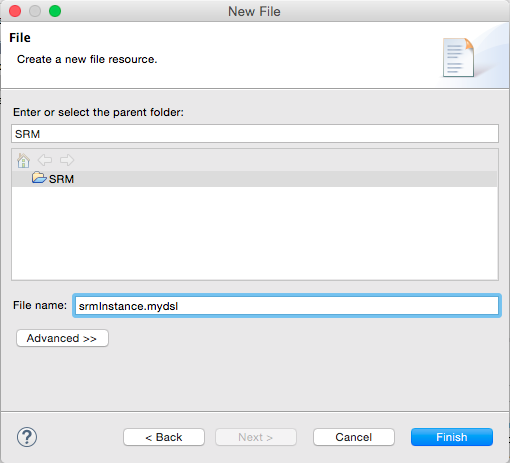
\includegraphics[scale=0.7]{images/creatingSRMDSL}
	\fautor
\end{figure}


\begin{figure}[!h]
	\centering
	% Requires \usepackage{graphicx}
	\caption{Editor Textual para instanciar o metamodelo SRM.}
	\label{fig:editor_SRM_metamodel_ECORE}
	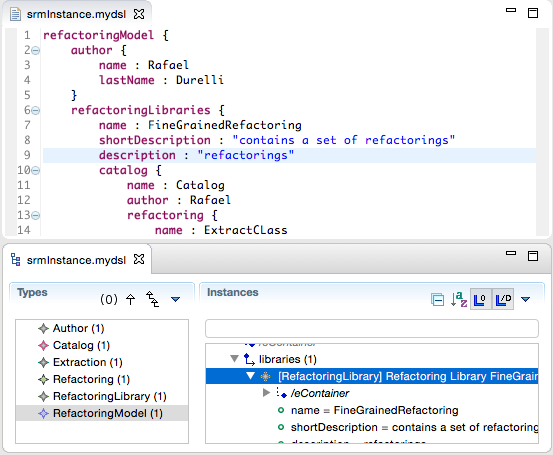
\includegraphics[scale=0.65]{images/dsl_SRM_ECORE}
	\fautor
\end{figure}

\begin{figure}[!h]
	\centering
	% Requires \usepackage{graphicx}
	\caption{Menu para enviar instâncias do metamodelo SRM.}
	\label{fig:editor_SRM_metamodel_ECORE_menu}
	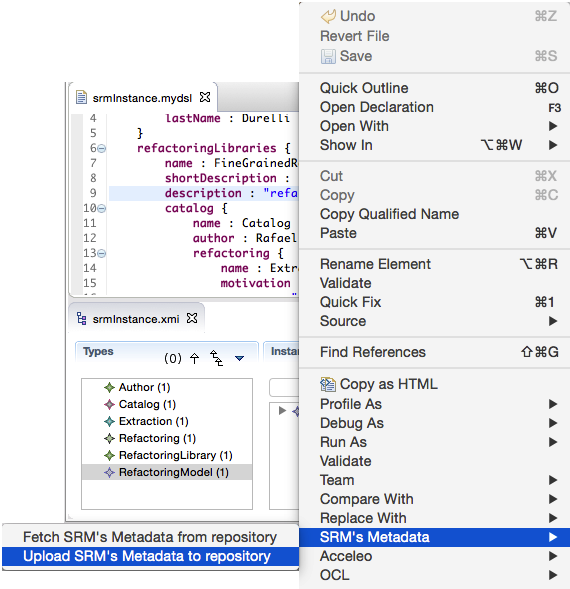
\includegraphics[scale=0.65]{images/SRM_Upload_Image}
	\fautor
\end{figure}

%No Código-fonte~\ref{lst:dsl_part_5} as sintaxes concretas das metaclasses \texttt{Operation}, \texttt{PreCondition} e \texttt{PostCondition} são definidas. A sintaxe concreta da metaclasse \texttt{Operation} inicia com a palavra-chave \texttt{operation} seguida por um \aspas{\{}\ding{182}. Em seguida, deve-se especificar qual a linguagem que a operação/refatoração será escrita. \texttt{Language} é uma enumeração (\textit{enum}) que está representado na linha 24 do Código-fonte~\ref{lst:dsl_part_5}. A linha 5 representa a sintaxe concreta para especificar o \aspas{corpo} da operação/refatoração propriamente dita \ding{184}. Na linha 8 a sintaxe concreta da metaclasse \texttt{PreCondition} é definida. A sintaxe concreta inicia com a palavra-chave \texttt{preCondition} seguida por um \aspas{\{}\ding{182}, \texttt{context}, \texttt{language} e \texttt{body}. A sintaxe concreta da metaclasse \texttt{PostCondition} é definida nas linhas 16 até 23. Note que a sintaxe é similar à sintaxe definida na metaclasse \texttt{PreCondition}. A partir das gramáticas da DSL apresentadas XText gera um editor textual no ambiente de desenvolvimento Eclipse IDE. Esse editor provê para a KDM-RE \textit{highlighting} de sintaxe, \textit{code completion} e \textit{code navigation}. O editor resultante pode ser observado na Figura~\ref{fig:editor_SRM_metamodel_ECORE}.


%Identificar e reutilizar artefatos em nível de modelos é uma limitação hoje em dia~\cite{Rocco_2015}. Essa limitação faz com que modernizadores geralmente tenham que recriar soluções já existentes, tais como: metamodelos, transformações, etc, diminuindo assim a produtividade e benefícios defendidos pelo MDE. Dessa forma, para facilitar e promover o compartilhamento e o reúso de refatorações por meio do metamodelo SRM é necessário uma forma que permita que modernizadores possam enviar, analisar e reutilizar as refatorações instanciadas para um artefato central. Assim, outros modernizadores podem contribuir com a criação de um conjunto de metadados sobre refatorações para que outros modernizadores possam pesquisar, identificar e reutilizar refatorações em seu projeto durante a modernização. 

%Neste contexto, um repositório foi criado para persistir instâncias do metamodelo SRM, onde tais instâncias representam metadados sobre refatorações que podem ser pesquisas e reutilizadas por outros modernizadores. Na Figura~\ref{fig:repositorio} é apresentado o diagrama de entidade e relacionamento do repositório. É importante observar que cada tabela apresentado nessa figura representa uma metaclasse do metamodelo SRM. Por exemplo, a metaclasse \texttt{Refactoring} apresentada na Figura~\ref{fig:meta_modelo_SRM} equivale a entidade \texttt{Refactoring} ilustrada na Figura~\ref{fig:repositorio}. 

%\begin{figure}[!h]
%	\centering
%	\caption{Diagrama de Entidade e Relacionamento do Metamodelo SRM.}
%	\label{fig:repositorio}
%	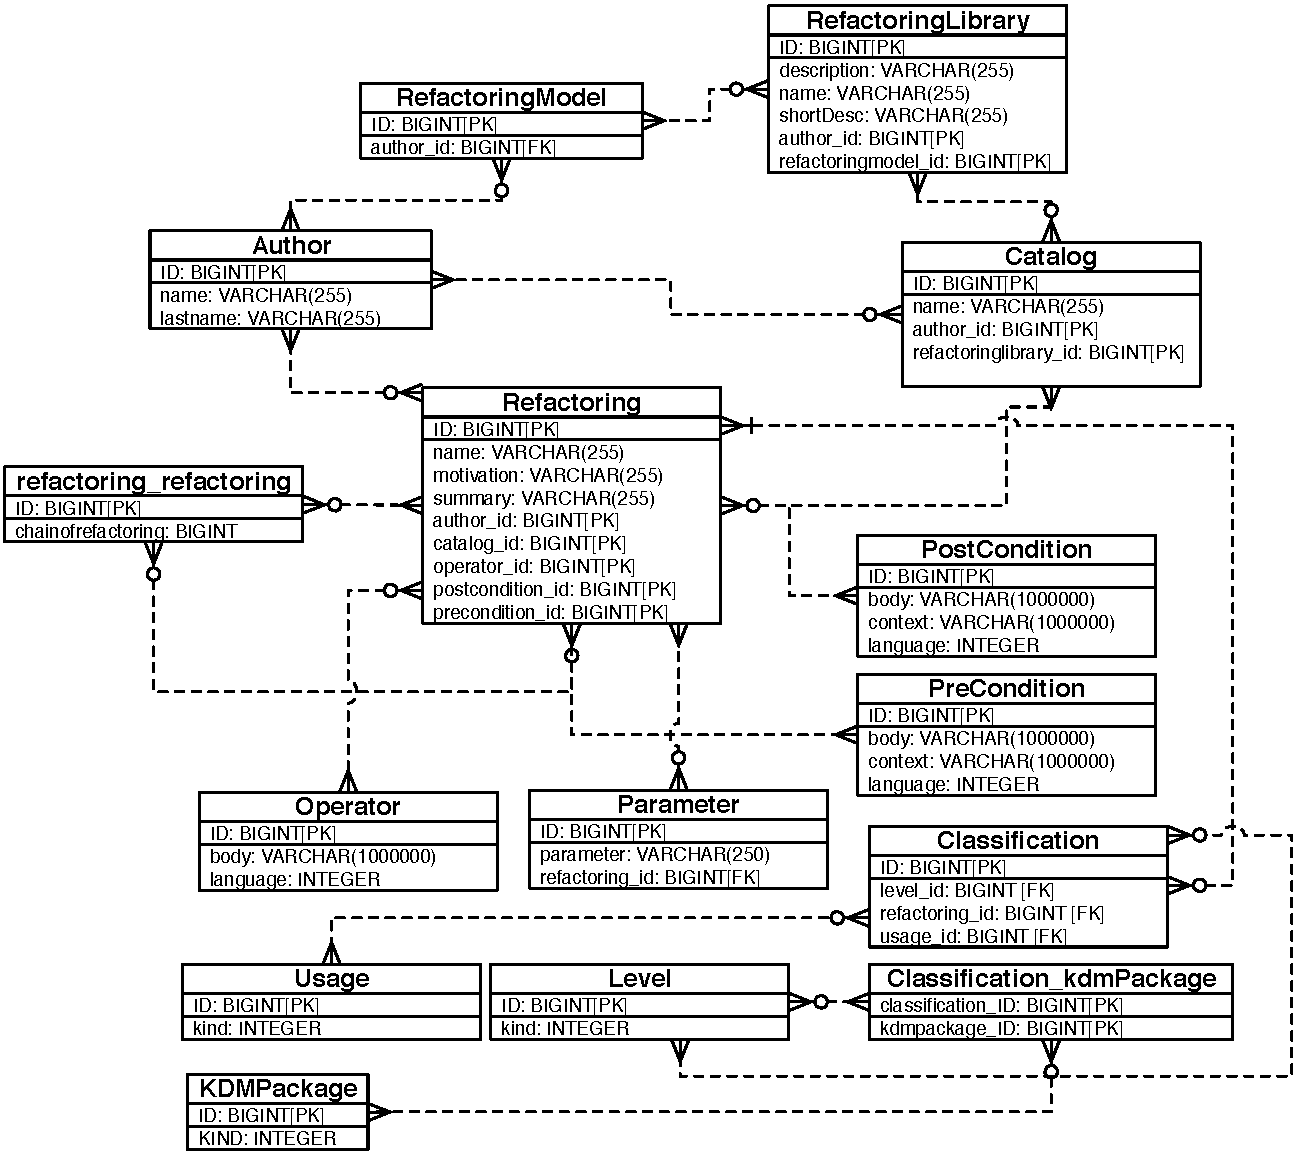
\includegraphics[scale=0.5]{images/ERD_refactoring}
%	\fautor
%\end{figure}

Para utilizar a DSL primeiramente o engenheiro de modernização precisa criar um arquivo com a extensão \aspas{.mydsl}. A KDM-RE fornece um \textit{wizard} para criar esse arquivo como apresentado na Figura~\ref{fig:creatingSRMDSL}. Por meio desse \textit{wizard} o engenheiro de modernização deve especificar um nome para o arquivo e também deve especificar a extensão do arquivo como \aspas{.mydsl}. É importante que o engenheiro de modernização especifique a extensão correta do arquivo, ou seja, \aspas{.mydsl}. Essa extensão é utilizada para o módulo do SRM identificar que o arquivo criado é na verdade a DSL definida na gramática apresentada nos Códigos-fontes~\ref{lst:dsl_part_1} -~\ref{lst:dsl_part_5}. No exemplo apresentado na Figura~\ref{fig:creatingSRMDSL} o arquivo foi definido como \texttt{srmInstance.mydsl}. Dessa forma, a KDM-RE automaticamente irá criar um editor para auxiliar o engenheiro de modernização a especificar uma refatoração utilizando as sintaxes da DSL. Após a criação do arquivo \texttt{srmInstance.mydsl} o engenheiro de modernização deve começar a especificar uma determinada refatoração como apresentado na Figura~\ref{fig:editor_SRM_metamodel_ECORE}. 


Adicionalmente, a KDM-RE fornece uma maneira de armazenar e compartilhar instâncias do metamodelo SRM. O principal objetivo é fazer com que refatorações definidas utilizando o metamodelo SRM sejam reutilizadas em projetos que utilizam o metamodelo KDM. Assim, após definir uma instância do metamodelo SRM utilizando a DSL, por meio do editor apresentado na Figura~\ref{fig:editor_SRM_metamodel_ECORE}, o engenheiro de modernização deve enviar os metadados de uma determinada instância do SRM para um repositório remoto. Esse processo é realizado por meio de um menu denominado \texttt{Upload SRM's Metadata to repository} - para interagir com esse menu o engenheiro deve clicar com o botão direito no editor textual da DSL e escolher \texttt{SRM's Metadata} como apresentado na Figura~\ref{fig:editor_SRM_metamodel_ECORE_menu}. Transparentemente a KDM-RE irá converter a sintaxe e a semântica da DSL em um arquivo XMI como ilustrado no Código-fonte~\ref{lst:xml_srm_convertido}. Note que nesse código-fonte os códigos em ATL e OCL foram omitidos para facilitar o entender do arquivo XMI. 

É importante também observar que cada marcação no XMI representa uma metaclasse do metamodelo SRM. Por exemplo, \aspas{\textbf{<refactoringModel>}}, \aspas{\textbf{<libraries>}}, \aspas{\textbf{<catalogs>}} e \aspas{\textbf{<refactorings>}} estão em conformidades com as metaclasses \texttt{RefactoringModel}, \texttt{RefactoringLibrary}, \texttt{Catalog} e \texttt{Refactoring} do SRM, respectivamente. Em seguida, esse arquivo XMI é lido, enviado e armazenados em um repositório remoto para ser posteriormente manipulado. 

\begin{lstlisting}[language=XML, frame=single, basicstyle={\scriptsize}, mathescape=true, label={lst:xml_srm_convertido}, caption={Arquivo XMI representando a instância do SRM.}]
<?xml version="1.0" encoding="ASCII"?>
<refactoringModel:RefactoringModel xmi:version="2.0" xmlns:xmi="http://www.omg.org/XMI" xmlns:xsi="http://www.w3.org/2001/XMLSchema-instance" xmlns:refactoringModel="http://refactoringModel/1.0">
  <libraries name="FineGrainedRefactoring" shortDescription="contains a set of refactorings" description="refactorings">
    <catalogs name="Catalog" author="//@author">
      <refactorings name="ExtractCLass" motivation="Motivation" summary="Summary">
        <preCondition context="TO BE DEFINED" language="OCL" body="TO BE DEFINED"/>
        <postCondition context="TO BE DEFINED" language="OCL" body="TO BE DEFINED"/>
        <operation body="TO BE DEFINED"/>
      </refactorings>
    </catalogs>
  </libraries>
  <author name="Rafael" lastName="Durelli"/>
</refactoringModel:RefactoringModel>
\end{lstlisting}


 A KDM-RE também fornece uma maneira de visualizar todas as instâncias do SRM disponíveis no repositório remoto. Essa opção é realizada por meio do menu \texttt{SRM's Metadata} e em seguida \texttt{Fetch SRM's Metadata from repository} (ver Figura~\ref{fig:editor_SRM_metamodel_ECORE_menu}). Após clicar no menu \texttt{Fetch SRM's Metadata from repository} a Figura~\ref{fig:download_kDM_re_repository} é apresentada, a qual fornece a visualização de todas as instâncias do metamodelo SRM disponíveis para serem reutilizadas. Nesse figura pode ser observado que existem seis instâncias do metamodelo SRM: \texttt{PullUpMethodUnit}, \texttt{ExtractClassUnit}, \texttt{PushDownStorableUnit}, \texttt{PushDownMethodUnit}, \texttt{InLineClassUnit} e outra \texttt{ExtractClassUnit}. KDM-RE permite que o engenheiro de software visualize a refatoração para cada instância do metamodelo SRM. Por exemplo, se o engenheiro almejar visualizar a refatoração escrita em ATL ele deve então selecionar uma determinada instancia do SRM e clicar no botão \texttt{VIEW}. Assim, a refatoração escrita em ATL será apresentada em uma área de texto como ilustrado na parte inferior da Figura~\ref{fig:download_kDM_re_repository}. Após escolher uma determinada instância do metamodelo SRM, o botão \texttt{DOWNLOAD} deve ser clicado para realizar a transferência da instância do metamodelo SRM e reutilizar em seu projeto. 

\begin{figure}[!h]
	\centering
	% Requires \usepackage{graphicx}
	\caption{Visão das instâncias do metamodelo SRM disponíveis no repositório.}
	\label{fig:download_kDM_re_repository}
	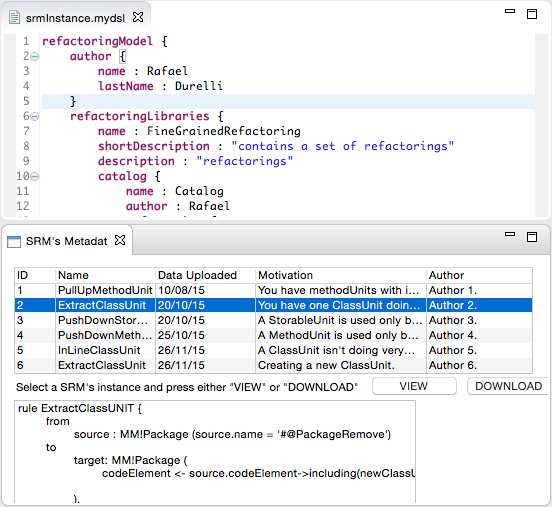
\includegraphics[scale=0.7]{images/DOWNLOAD_KDM_RE}
	\fautor
\end{figure}


\subsection{Módulo de Sincronização}

Nessa seção é apresentado um módulo desenvolvido para fornecer suporte a abordagem KDM-SInc ver Figura~\ref{fig:kdm_sinc} Capítulo~\ref{chapter:Abordagem_de_sincronizacao}. Como apresentado nos Capítulos~\ref{chapter:adm_kdm} e~\ref{chapter:Abordagem_de_sincronizacao} o metamodelo KDM contém pacotes heterogêneos que são utilizados para representar diferentes artefatos de um sistema. Assim, é importante manter uma determinada instância do metamodelo KDM consistente e sincronizada após a aplicação de refatorações. 

Como apresentado no Capítulo~\ref{chapter:Abordagem_de_sincronizacao} a abordagem KDM-SInc contém três principais passos. Para auxiliar a elaboração do módulo de sincronização técnicas, \textit{framework} e API foram utilizadas. O primeiro passo foi implementando utilizando o \textit{framework} EMFCompare\footnote{https://www.eclipse.org/emf/compare/}. Esse \textit{framework} foi utilizado e estendido para comparar instâncias do metamodelo KDM. Mais especificadamente EMFCompare foi utilizado para comparar uma instância do metamodelo KDM refatorada (KDM direito) com uma instância do metamodelo KDM não refatorada (KDM esquerdo). Essa comparação é importante para identificar quais instâncias foram afetadas, bem como quais operações foram realizadas pela refatoração (\texttt{add}, \texttt{delete} e \texttt{change}). 

No segundo passo da abordagem KDM-SInc um motor de busca foi desenvolvido. Esse motor de busca utiliza como base o algoritmo DFS juntamente com um conjunto de expressões definidas em XPath que são executadas em uma instância do metamodelo KDM para obter todos os pacotes/visões do KDM. No terceiro passo propagações são realizadas. Tais propagações foram definidas e implementas por meio de um motor de propagação. Esse motor utiliza um conjunto de regras pré-definidas e implementadas em ATL. Essas regras são disparadas de acordo com alterações identificadas no primeiro e no segundo passo da abordagem KDM-SInc. Por exemplo, as regras em ATL são um conjunto de transformações que foram definidas de acordo com a instância alterada (\texttt{Package}, \texttt{ClassUnit}, \texttt{MethodUnit}, \texttt{StorableUnit}, etc) e sua operação atômica (\texttt{add}, \texttt{delete} e \texttt{change}). No Capítulo~\ref{chapter:Abordagem_de_sincronizacao} mais especificadamente nas Tabelas~\ref{tab:propagacaoes_kdm_sinc_package},~\ref{tab:propagacaoes_kdm_sinc_classUnit},~\ref{tab:propagacaoes_kdm_sinc_StorableUnit} e~\ref{tab:propagacaoes_kdm_sinc_method} pode-se visualizar com mais detalhes essas regras.

O módulo de sincronização foi implementado para ser executado de forma transparente para o engenheiro de software. Porém, para que esse módulo de sincronização seja executado uma condição primordial deve ser satisfeita - a instância do metamodelo KDM deve representar outros artefatos do sistema, não apenas o código-fonte por meio do pacote \texttt{Code} do KDM. O módulo de sincronização verifica se a instância do metamodelo KDM a ser sincronizada e propagada contém abstrações dos outros pacotes do metamodelo KDM, ou seja, assegura-se os pacotes do KDM estão sendo utilizados para representar outros artefatos, tais como: banco de dados, GUI, elementos estruturais, etc. Caso essa condição seja satisfeita o módulo de sincronização pode então ser executado.

Todas as propagações definidas nesse módulo foram criadas para serem disparadas após a aplicação de específicas alterações na instancia do metamodelo KDM. Algumas propagações podem ser realizadas sem a interferência do engenheiro de software, no entanto, existem propagações que precisam de informações importantes para realizar consistentemente a propagação. Assim, algumas propagações podem ser realizadas de forma totalmente automática, enquanto outras precisam de algumas informações antes de executar a propagação propriamente dita.

Por exemplo, considere a Figura~\ref{fig:kdm_re_wizard_extract_class} apresentada neste capítulo, onde o engenheiro de software irá aplicar a refatoração \texttt{Extract ClassUnit}. Além disso, considere também que para o pacote \texttt{Data} do KDM esta sendo utilizado para representar entidades de banco de dados, tais como tabelas, colunas, chaves-primárias, etc.

Como já salientado o módulo de sincronização utiliza o \textit{framework} EMFCompare. Como apresentado no Capítulo~\ref{chapter:Abordagem_de_sincronizacao} esse \textit{framework} realiza três sub-passos: (\textit{i}) \textit{Matching}, (\textit{ii}) \textit{Diffing} e (\textit{iii}) Análise dos \textit{Diffs} como apresentado na Figura~\ref{fig:diff_emf_compare} do Capítulo~\ref{chapter:Abordagem_de_sincronizacao}.

No primeiro sub-passo o módulo de sincronização, utiliza duas instâncias do metamodelo KDM - uma instância original (\aspas{KDM esquerdo}) denominada \textbf{versão 1} e uma instância refatorada (\aspas{KDM direito}) \textbf{versão 2}. Dado essas duas instâncias os correspondentes elementos nessas duas versões do metamodelo KDM são identificados. Os correspondentes elementos são identificados por meio de identificadores únicos tais como XMI IDs. Para cada elemento correspondente identificado, ou não identificado, o módulo de sincronização cria um elemento \textit{match} que é utilizado no sub-passo seguinte.

Em seguida, no segundo sub-passo, \textit{Diffing}, todos os correspondentes elementos identificados são examinados para identificar diferenças em seus meta-atributos. Para cada diferença identificada o módulo de sincronização cria um objeto \textit{diff}, o qual descreve com precisão cada diferença entre os correspondentes elementos. Instâncias de metaclasses que não contêm elementos correspondentes em ambas as versões (\aspas{KDM esquerdo} e \aspas{KDM direito}) são consideradas adicionadas ou deletadas (\texttt{add} e \texttt{delete}) - a operação é identificada dependendo da direção, por exemplo, se uma instância de uma metaclasse apenas existe do lado direito (\aspas{KDM direito}) essa instância foi adicionada, por outro lado, se uma instância apenas existe do lado esquerdo (\aspas{KDM esquerdo}) essa instância foi deletada. Meta-atributos que forem alterados durante a refatoração representam a operação \texttt{change}. Em seguida o terceiro sub-passo, Análise dos \textit{Diffs} é executado. Nesse sub-passo todos os objetos \textit{diffs} criados anteriormente pelo módulo de sincronização são analisados.


Como apresentado no Capítulo~\ref{chapter:catalogo_refactoring_KDM} a refatoração \texttt{Extract ClassUnit} é realizada por um conjunto de duas operações atômicas: \texttt{add} e  \texttt{delete}. Dessa forma, o módulo de sincronização identifica que a refatoração \texttt{Extract ClassUnit} executou um conjunto de operações atômica (\texttt{add} e  \texttt{delete}) e cria uma lista para ser utilizada no passo seguinte. No contexto da refatoração \texttt{Extract ClassUnit} apresentada na Figura~\ref{fig:kdm_re_wizard_extract_class} as seguintes operações foram realizadas: 

\begin{itemize}
\item \texttt{add} uma instância de \texttt{ClassUnit} denominada \texttt{Document};
\item \texttt{delete} uma instância de \texttt{StorableUnit} denominada CPF da \texttt{ClassUnit} \texttt{Cliente}
\item \texttt{add} uma instância de \texttt{StorableUnit} na \texttt{ClassUnit} \texttt{Document};
\item \texttt{add} uma instância de \texttt{StorableUnit} do tipo \texttt{Document} na \texttt{ClassUnit} \texttt{Cliente};
\item \texttt{add} duas instância de \texttt{MethodUnit} para representar os métodos assessores na \texttt{ClassUnit} \texttt{Cliente}
\end{itemize}

Em seguida o módulo de sincronização executa o algoritmo DFS para identificar todas as metaclasses que precisam ser sincronizadas/atualizadas após a aplicação da refatoração. Esse algoritmo utiliza como entrada a lista criada no passo anterior. Expressões definidas em XPath são utilizadas para navegar em todas as visões da instância do metamodelo KDM. Maiores informações de como o algoritmo é adaptado e executado para instâncias do metamodelo KDM podem ser obtidas no Capítulo~\ref{chapter:Abordagem_de_sincronizacao}. Ao término da execução desse algoritmo, o mesmo irá criar uma lista que contém todas as instâncias das metaclasses afetadas na refatoração. 
   

O terceiro passo da abordagem KDM-SInc objetiva realizar as mudanças e propagações necessários para manter uma determinada instância do metamodelo KDM sincronizada e consistente. Utilizando a lista de operações realizadas na refatoração e a lista que possui os elementos afetados na refatoração o módulo de programação utiliza um conjunto de regras pré-definidas para realizar a propagação. Todas as propagações são apresentadas nas Tabelas~\ref{tab:propagacaoes_kdm_sinc_package},~\ref{tab:propagacaoes_kdm_sinc_classUnit},~\ref{tab:propagacaoes_kdm_sinc_StorableUnit} e~\ref{tab:propagacaoes_kdm_sinc_method}. Na Figura~\ref{fig:efeitoPropagacaoKDMSINC} é apresentado duas instâncias do metamodelo KDM. A instância apresentada do lado esquerdo equivale a instância antes de aplicar o módulo de sincronização. A instância do lado direito representa a uma instância do metamodelo KDM sincronizada e propagada de acordo os passos e regras definidas pela abordagem KDM-SInc nas Tabelas~\ref{tab:propagacaoes_kdm_sinc_package},~\ref{tab:propagacaoes_kdm_sinc_classUnit},~\ref{tab:propagacaoes_kdm_sinc_StorableUnit} e~\ref{tab:propagacaoes_kdm_sinc_method}.


\begin{figure}[!h]
	\centering
	% Requires \usepackage{graphicx}
	\caption{Instância antes e após a abordagem KDM-SInc..}
	\label{fig:efeitoPropagacaoKDMSINC}
	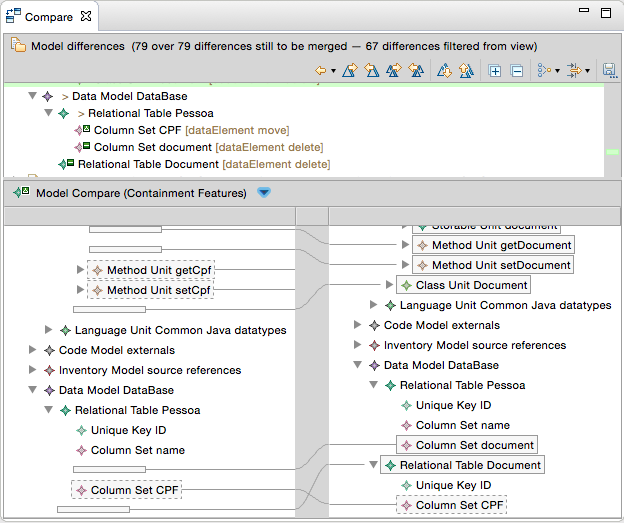
\includegraphics[scale=0.7]{images/propagacaoKDMEfeito}
	\fautor
\end{figure}


%Como observado a instância apresentada do lado direito da Figura~\ref{fig:efeitoPropagacaoKDMSINC} representa a instância do metamodelo KDM sincronizada e propagada. 


%A sincronização é importante para o metamodelo KDM uma vez que o mesmo possui metaclasses que contêm conexões diretas com outras metaclasses de outras visões/artefatos do KDM. Assim, manter a instância do metamodelo KDM sincronizado e consistente após a aplicação de uma refatoração é importante. 

%No contexto desta Tese, como apresentado no Capítulo~\ref{chapter:catalogo_refactoring_KDM} as refatorações que são definidas e adaptadas para o metamodelo KDM são refatorações de baixa granularidade e que são aplicadas diretamente na camada \texttt{Code} do metamodelo KDM. Porém, uma determinada refatoração pode demandar outras modificações que deveriam ser realizadas em outros camadas/visões do metamodelo KDM para mantê-lo consistente e sincronizado. Por exemplo, considere a refatoração \textit{Rename Package} - o nome de um determinado pacote é alterado de PacoteX para PacoteY, se uma instância da metaclasse \texttt{Layer}\footnote{Metaclasse definida no pacote \texttt{Structure} do metamodelo KDM para representar camadas em nível arquitetural.} é utilizada para representar o pacote em nível arquitetural, então essa mesma instância da metaclasse \texttt{Layer} também deve-se ser renomeada. 

%Diferentemente da atividade de refatoração apresentada no Capítulo~\ref{chapter:catalogo_refactoring_KDM} onde o engenheiro de modernização precisa escolher qual refatoração aplicar na instância do metamodelo KDM ou reutilizar um refatoração utilizando o metamodelo SRM apresentado no Capítulo~\ref{chapter:Toward_a_Refactoring_Metamodel_for_KDM}, esse passo utiliza um conjunto de regras pré-definidas que são iniciadas de acordo a(s) refatoração(ões) aplicada(s) na instância do metamodelo KDM. Mais especificadamente, todas as propagações especificadas nesse passo são pré-definidas para serem disparadas após a aplicação de específicas refatorações. Algumas propagações são realizadas sem a interferência do engenheiro de modernização, no entanto, existem propagações que precisam de informações importantes para realizar consistentemente a propagação. Assim, algumas propagações podem ser realizadas de forma totalmente automática, enquanto outras precisam de algumas informações antes de executar a propagação propriamente dita.

%Esse passo da abordagem KDM-SInc utiliza um conjunto de regras pré-definidas para propagar todas as mudanças em uma instância do metamodelo KDM com o intuito de mantê-lo consistente e sincronizado com todas as visões/artefatos. Todas as propagações são definidas com base nas mudanças realizadas em um determinada instância de metaclasses do metamodelo KDM. A abordagem KDM-SInc 

%Por exemplo, considere a Figura~\ref{fig:extractClassRefactoring} onde o engenheiro de modernização está aplicando a refatoração \texttt{Extract ClassUnit} em uma instância de \texttt{ClassUnit} denominada \texttt{Pessoa}. O primeiro passo do módulo de sincronização irá realiazar uma comparação entre a instância refatorada e a instância original do metamodelo KDM. Como apresentado no Capítulo X\change{mudar} a refatoração \texttt{Extract ClassUnit} é uma refatoração composta, assim, é necessário aplicar um conjunto de operações atômicas: \texttt{add}, \texttt{delete} e \texttt{change}.


\section{Considerações Finais}

Neste capítulo é apresentado a ferramenta KDM-RE. A KDM-RE foi construída, de modo a ser utilizada em conjunto com os demais recursos oferecidos pelo ambiente de desenvolvimento Eclipse IDE. Os \textit{plug-ins} da KDM-RE são organizados em módulos de acordo com a sua funcionalidade. Os três principais módulos são: (\textit{i}) módulo de refatoração, (\textit{ii}) módulo do SRM e (\textit{iii}) módulo de sincronização. 

O primeiro módulo é responsável por criar uma infraestrutura que permita o engenheiro de software aplicar refatorações em nível de modelos no contexto do metamodelo KDM. O engenheiro de software pode aplicar as refatorações no metamodelo KDM por meio de duas principais interfaces, a primeira denominada \textit{model browser} onde o engenheiro tem uma visão de árvore da instância do metamodelo KDM e a segunda interface onde o engenheiro pode aplicar refatorações diretamente em diagramas de classe da UML. Embora o engenheiro utilize diagrama de classe na segunda interface as refatorações são aplicadas de forma transparente na instância do metamodelo KDM - o diagrama de classe é utilizado apenas para extrair metadados (nome da classe, nome do atributo, tipo do atributo, etc) que são enviadas como entrada para a refatoração pré-definida em ATL.

O segundo módulo é responsável por oferecer um DSL para instanciar o metamodelo SRM apresentado no Capítulo~\ref{chapter:Toward_a_Refactoring_Metamodel_for_KDM}. Além disso o módulo do SRM fornece uma forma de reutilizar e compartilhar refatorações por meio de instâncias do metamodelo SRM. Para permitir o reúso e compartilhamento de refatorações um repositório remoto foi criado. Esse repositório remoto é dedicado para executar solicitações RESTful. Instâncias do metamodelo SRM são enviadas e recebidas por meio da API RESTful. JPA e o banco de dados MySQL foram utilizados para realizar as persistências das instâncias do metamodelo SRM.

Finalmente o terceiro módulo é responsável por implementar a abordagem apresentada no Capítulo~\ref{chapter:Abordagem_de_sincronizacao}. Esse módulo tem como objetivo propagar e sincronizar uma determinada instância do metamodelo KDM após a aplicação de refatorações. Como o metamodelo KDM possui um conjunto de pacotes para representar diferentes artefatos é importante manter a instância e todos os outros artefatos sincronizados após a aplicação de refatorações.